% Intended LaTeX compiler: pdflatex
\documentclass[a4j, 11pt]{jarticle}
\usepackage[dvipdfmx]{graphicx}
\usepackage[dvipdfmx]{color}
\usepackage{indentfirst}
\usepackage{fancyhdr}
\usepackage{lastpage}
\usepackage{amsmath, amssymb, bm}

\makeatletter
\author{201611350 江畑 拓哉}
\date{2017年10月16日}
\title{演習課題2}

\pagestyle{fancy}

% headers & footers
\lhead{数理アルゴリズム \@title 提出日:\@date\\\@author}
\chead{}
\rhead{}
\lfoot{}
\cfoot{\thepage /\pageref{LastPage}}
\rfoot{}
\renewcommand{\headrulewidth}{0pt}
\renewcommand{\footrulewidth}{0pt}
\makeatother


\begin{document}

\section{課題1}
\label{sec:org325f858}
\subsection{}
\label{sec:org4ef2062}
 次に示す配列 a, b からなるデータ列を配列 a の i 番目の要素 a i を横軸に,配列 b の i 番目の要素 b i を縦軸としたグラフを描画せよ.その際, plot 関数を使うこと.\\
\begin{verbatim}
plot(a, b)
\end{verbatim}

\begin{center}
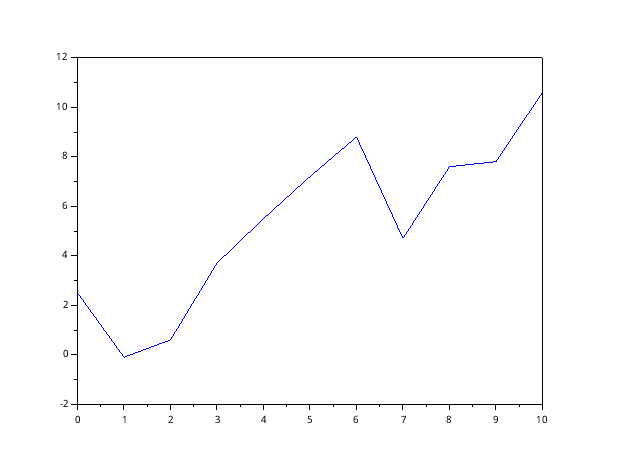
\includegraphics[width=10cm]{./1-1.png}
\end{center}
\subsection{}
\label{sec:org7ee49da}
 (1-1) で用いたデータ列を使用して,破線と任意のマーカーを用いてグラフを描画せよ.\\
\begin{verbatim}
plot(a, b, '--*')
\end{verbatim}

\begin{center}
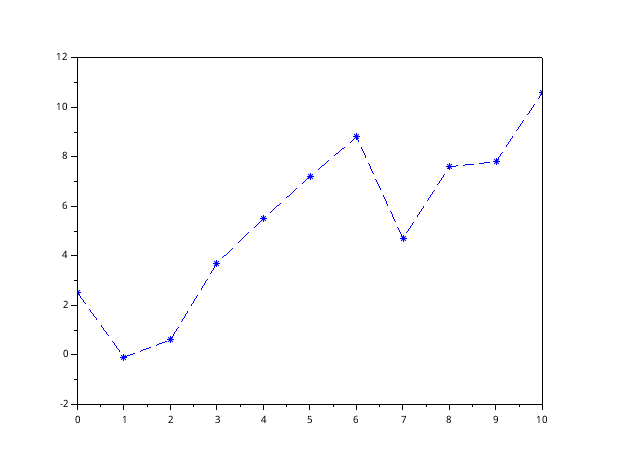
\includegraphics[width=10cm]{./1-2.png}
\end{center}
\subsection{}
\label{sec:org4a21f1d}
 (1-2) で描画したグラフに対して,タイトルと軸ラベルを表示せよ.\\
\begin{verbatim}
--> plot(a, b, '--*')

--> title('Plot Test')

--> xlabel('ai')

--> ylabel('bi')
\end{verbatim}

\begin{center}
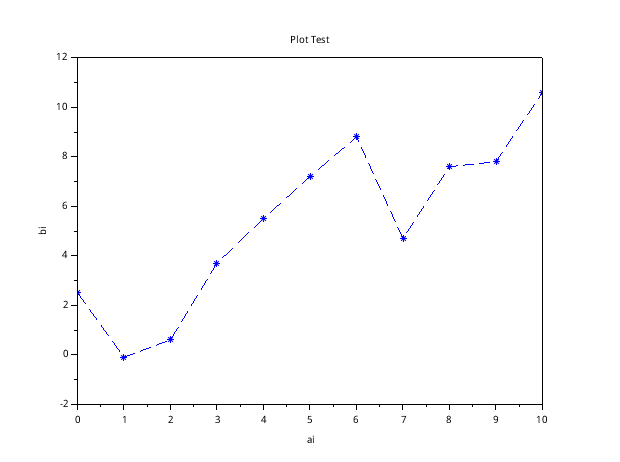
\includegraphics[width=10cm]{./1-3.png}
\end{center}
\section{課題2}
\label{sec:org7735e0d}
次に示すベクトルからなるデータ列を片対数グラフで描画せよ.また,通常のグラフも描画し,片対数グラフと比較して違いを考察せよ.\\
\begin{verbatim}
--> a = [0, 1, 2, 3, 4, 5, 6, 7, 8, 9, 10]
--> b = [0.5, 0.6, 1.5, 1.4, 1.3, 360, 180, 160, 130, 200, 80]
--> plot2d('nn', a, b)
\end{verbatim}

\begin{center}
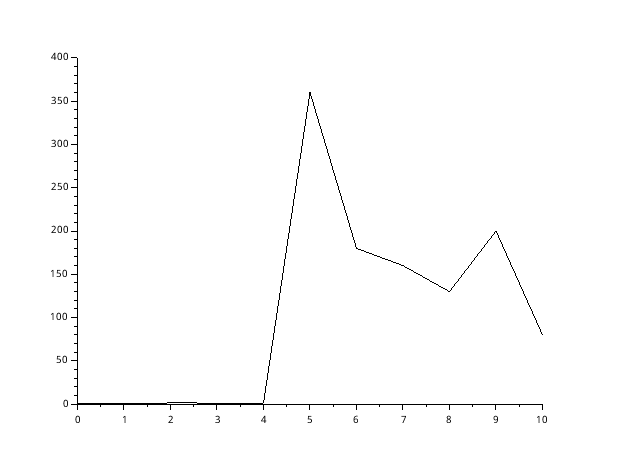
\includegraphics[width=10cm]{./2-no-kata.png}
\end{center}

\begin{verbatim}
--> plot2d('nl', a, b)
\end{verbatim}
\begin{center}
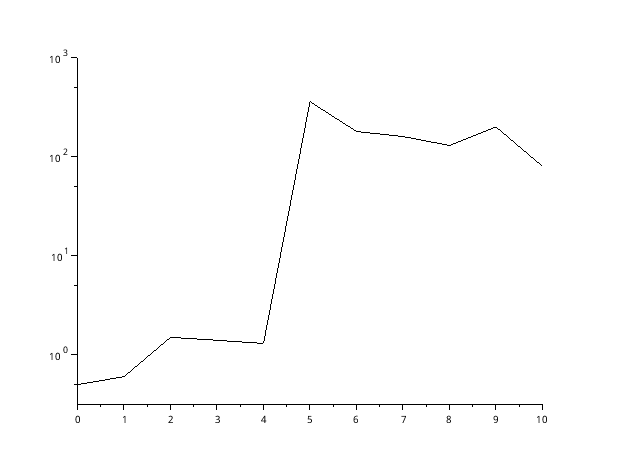
\includegraphics[width=10cm]{./2-kata.png}
\end{center}
\section{課題3}
\label{sec:org6492a9e}
\(z = e^{x^2+y^2}\) のグラフを surf 関数を用いて描画せよ.\\
\begin{verbatim}
surf(linspace(-0.5, 0.5, 100), linspace(-0.5, 0.5, 100), ..
exp(repmat((linspace(-0.5, 0.5, 100))^2, 100, 1) + ..
(repmat((linspace(-0.5, 0.5, 100))^2, 100, 1))'));
\end{verbatim}
\begin{center}
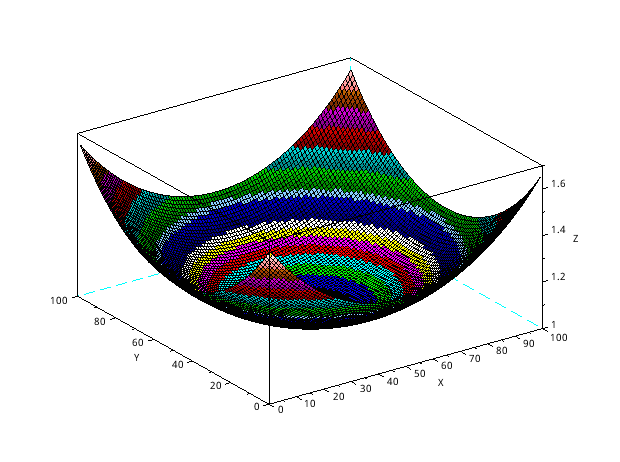
\includegraphics[width=10cm]{./3.png}
\end{center}
\section{課題4}
\label{sec:org6799164}
\subsection{}
\label{sec:org14396b3}
x 軸の範囲,分割点数および係数をパラメータとして多項式関数の描画を行う Scilab の関数を作成せよ.\\
\begin{verbatim}
function [] = createGraph(xfrom, xto, m, a)
x = linspace(xfrom, xto, m);
y = zeros(1, m);
n = size(a, 2) - 1;
for i=1:n
    y = (y + a(i)) .* x;
end
y = y + a(n + 1);
plot(x, y)
endfunction
\end{verbatim}
\subsection{}
\label{sec:org6e6c73a}
\(y=-2x^3+x^2+2x+3\) \((-3\leq x\leq 3)\) および\\
\(y = 0.4x^4 - 4.7 x^2 + 4.1x - 4\) \(( -4 \leq x \leq 4)\) のグラフを描画せよ.\\
\begin{verbatim}
--> createGraph(-3, 3, 30, [-2, 1, 2, 3])
--> createGraph(-4, 4, 30, [0.4, 0, -4.7, 4.1, -4])
\end{verbatim}
\begin{center}
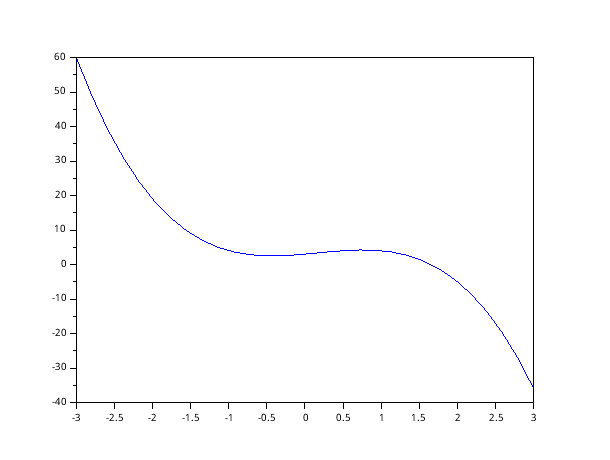
\includegraphics[width=10cm]{./4-1.png}
\end{center}
\begin{center}
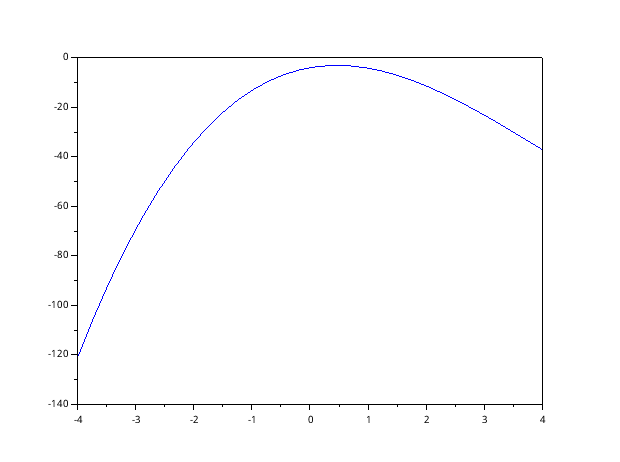
\includegraphics[width=10cm]{./4-2.png}
\end{center}
\end{document}
